\documentclass{article}
\usepackage{color}
\usepackage{tikz}
\usepackage{float}
\usepackage{tabularx}
\usepackage{amsmath}
\usepackage{amssymb}
\usepackage{listings}
\usepackage{enumitem}
\usepackage{syntax}
\usepackage{csquotes}
\usepackage{pgfplots}
\usepackage[backend=biber]{biblatex}
\addbibresource{references.bib}

\usetikzlibrary{chains}
\makeatletter
\tikzset{
  on chain/.append code={
    \ifnum\c@pgf@counta=1\relax
      \tikzset{every first on chain/.try}%
    \fi
  },
  start chain/.append code={%
    \edef\pgf@marshal{\noexpand\tikzset{execute at end scope={\noexpand\xdef\noexpand\tikzpreviouschain{\tikz@lib@chain@name}}}}%
    \pgf@marshal
  }
}
\def\listset{\pgfqkeys{/List}}
\tikzset{
  raw sort entry/.style={rectangle, thick, draw, font=\strut,text depth=+0pt,minimum width=+1.2em, inner xsep=+0pt},
  sort entry black/.style={raw sort entry, black, fill=white},
  sort entry blackgray/.style={raw sort entry, black, fill=gray!25},
  s1/.style={raw sort entry, fill=yellow!30},
  s2/.style={raw sort entry, fill=green!20},
  s3/.style={raw sort entry, fill=red!25},
  g/.style={raw sort entry, fill=lightgray}
}
\listset{
  chain name/.initial=,
  do/.style={
    /utils/exec={\begin{scope}[start chain=\pgfkeysvalueof{/List/chain name}]},
    int/do/.list={#1},
    /utils/exec=\end{scope},
  },
  int/do/.code={%
    \pgfutil@ifnextchar[\tikz@List@int@@do{\tikz@List@int@@do[]}#1\pgf@stop
  }
}
\def\tikz@List@int@@do[#1]#2\pgf@stop{%
  \node[on chain={\pgfkeysvalueof{/List/chain name}},#1] {#2};
}

\usepackage{tikz}
\usetikzlibrary{automata,positioning}
\tikzset{
  gray box/.style={
    fill=gray!20,
    draw=gray,
    minimum width={2*#1ex},
    minimum height={2em},
  },
  annotation/.style={
    anchor=north,
  }
}


\definecolor{dkgreen}{rgb}{0,0.6,0}
\definecolor{gray}{rgb}{0.5,0.5,0.5}
\definecolor{mauve}{rgb}{0.58,0,0.82}


\lstset{frame=tb,
  numbers=left,
  stepnumber=1,
  language=Java,
  aboveskip=3mm,
  belowskip=3mm,
  showstringspaces=false,
  columns=flexible,
  basicstyle={\small\ttfamily},
  numberstyle=\color{gray},
  keywordstyle=\color{blue},
  commentstyle=\color{dkgreen},
  stringstyle=\color{mauve},
  breaklines=true,
  breakatwhitespace=true,
  tabsize=2,
  moredelim=**[is][\color{red}]{@}{@},
}

\setlength{\grammarindent}{12em}

%\renewcommand{\lstlistingname}{Algorithm}
%\newcommand{\tablerow}[4]{ #1 & #2 & #3 & #4\\}
\newcommand{\n}[0]{\\[\baselineskip]}
%\newcommand{\qa}[2]{\textbf{Q:} #1 \\ \textbf{A:} #2}
%\newcommand{\argument}[4]{\textbf{#1:} #2 \\ \textbf{#3:} #4}

\title{CS4202 Computer Architecture - Process Scheduling for Heterogeneous Systems}
\author{140011146}

\begin{document}

\maketitle

\section{Introduction}
CPU scheduling is vital for the multitasking environment of modern operating systems. Processes waiting for I/O can be switched out to prevent wasted CPU cycles, but any process can be pre-empted for better user interactivity, efficiency and fairness \cite{os}. As a result, it is important to understand the effects of scheduling on performance.
\n
First, a round-robin scheduling approach for CPUs is looked into, discussing how the approach works and where the approach performs well or poorly. 
\n
Next, a genetic algorithm was implemented to explore the search space of possible schedules with the GEM5 simulator on two benchmarks. The schedules produced by the genetic algorithm are then compared with both the default approach of the simulator and random schedules to gain an understanding of the scheduling optimisation space.

\section{Task 1 - Round-robin scheduling}
The round-robin CPU scheduling approach is similar to a simple First-Come First-Served scheduling approach, but all processes bursts are limited by a time quantum. This ensures fairness, giving all processes a chance to run, but comes at costs such as high waiting time and high turnaround time. There is much research going into optimising a round-robin scheduler, usually by means of calculating an optimal time quantum dynamically \cite{rr-paper3} \cite{rr-paper4} \cite{rr-paper2} or introducing some form of priority \cite{rr-paper5}.
\n
In the simple round-robin approach, a circular queue of processes that are ready to be executed is maintained by the scheduler. New processes join at the end of the queue. The scheduler chooses and removes the first process in the queue to run \cite{os}. Any running process will be pre-empted if they run longer than the time quantum. Processes that make block or finish before the time quantum are also moved off the CPU \cite{rr-paper}. A very long time quantum will effectively be the same as a FCFS approach, resulting in poor response and waiting time if there are processes with long bursts. On the other hand, a very short time quantum results in a large computational overhead of many context switches between the processes, wasting time and CPU cycles on context switching \cite{context-switch} rather than useful computation. Therefore, the length of the time quantum heavily impacts the performance of the round-robin approach and should be proportional to the time needed for context switches. For example, consider the following processes in the ready queue.
\begin{figure}[H]
\centering
\begin{tabular}{c c}
\textbf{Process} & \textbf{Burst time} \\
\hline
$P_{1}$ & 17 \\
$P_{2}$ & 3 \\
$P_{3}$ & 4 \\
\end{tabular}
\end{figure}
\noindent 
A time quantum of 3 would result in the following schedule and wait times:
\begin{figure}[H]
\centering
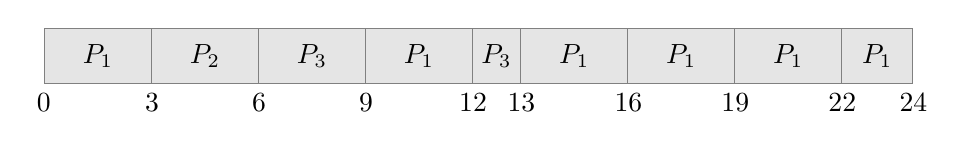
\begin{tikzpicture}[node distance=-0.5pt]
  \node [gray box=4.5] (p1) {\(P_{1}\)};
  \node [gray box=4.5, right=of p1] (p2) {\(P_{2}\)};
  \node [gray box=4.5, right=of p2] (p3) {\(P_{3}\)};
  \node [gray box=4.5, right=of p3] (p4) {\(P_{1}\)};
  \node [gray box=1.5, right=of p4] (p5) {\(P_{3}\)};
  \node [gray box=4.5, right=of p5] (p6) {\(P_{1}\)};
  \node [gray box=4.5, right=of p6] (p7) {\(P_{1}\)};
  \node [gray box=4.5, right=of p7] (p8) {\(P_{1}\)};
  \node [gray box=3, right=of p8] (p9) {\(P_{1}\)};

  \node [annotation] at (p1.south west) {0};
  \node [annotation] at (p1.south east) {3};
  \node [annotation] at (p2.south east) {6};
  \node [annotation] at (p3.south east) {9};
  \node [annotation] at (p4.south east) {12};
  \node [annotation] at (p5.south east) {13};
  \node [annotation] at (p6.south east) {16};
  \node [annotation] at (p7.south east) {19};
  \node [annotation] at (p8.south east) {22};
  \node [annotation] at (p9.south east) {24};
\end{tikzpicture}
\caption{Schedule with a time quantum of 3}
\end{figure}
\noindent Wait times:
\begin{itemize}
\item $P_{1}$: 7 time units
\item $P_{2}$: 3 time units
\item $P_{3}$: 9 time units
\end{itemize}
\noindent Average wait time = $19 / 3 = 6.33$ time units.
\\ Context switches = 8
\n
However, a time quantum of 10 would result in a much longer average wait time.
\begin{figure}[H]
\centering
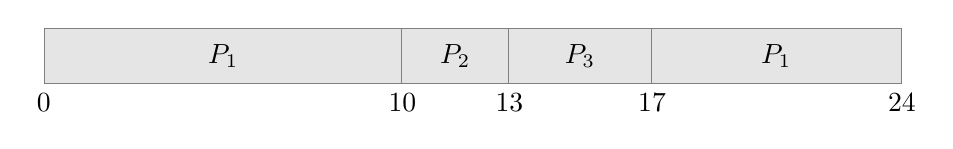
\begin{tikzpicture}[node distance=-0.5pt]
  \node [gray box=15] (p1) {\(P_{1}\)};
  \node [gray box=4.5, right=of p1] (p2) {\(P_{2}\)};
  \node [gray box=6, right=of p2] (p3) {\(P_{3}\)};
  \node [gray box=10.5, right=of p3] (p4) {\(P_{1}\)};

  \node [annotation] at (p1.south west) {0};
  \node [annotation] at (p1.south east) {10};
  \node [annotation] at (p2.south east) {13};
  \node [annotation] at (p3.south east) {17};
  \node [annotation] at (p4.south east) {24};
\end{tikzpicture}
\caption{Schedule with a time quantum of 10}
\end{figure}
\noindent Wait times:
\begin{itemize}
\item $P_{1}$: 7 time units
\item $P_{2}$: 10 time units
\item $P_{3}$: 13 time units
\end{itemize}
\noindent Average wait time = $30 / 3 = 10$ time units.
\\ Context switches = 3
\n
It can be seen from the example how the choice of time quantum affects the waiting time, response time and number of context switches required. If the context switches took 1 time unit and a time quantum of 3 time units was used, the CPU would waste 25\% of the time on switching between the processes. To make this worse, the small time quantum leads to an increased number of switches and a lot of computation will be wasted. To make good use of the processor, the time quantum should be a larger proportion compared to the time taken for context switching. Of course it also cannot be too big compared to the average burst time of processes or it will simply be a FCFS scheduler with little fairness. It is important to strike this balance of efficient CPU usage and fairness among ready processes. The long average waiting time is also an issue. Given $n$ processes in the ready queue with a time quantum of $t$, each process only gets $t$ time to run every $nt$ time units and must wait at most $(n - 1) \times t$ before each turn. 
\n
Round-robin is strong in cases where all processes bursts have similar lengths, or fairness is of greater importance to the system. For example in load balancing for parallel computation or time-sharing systems. However, problems with choosing an optimal time quantum and lack of ability to express priority, where some processes need a greater share of the processor than others means few systems would use a na\"{i}ve round-robin algorithm.
\n
There are many other more complex algorithms that are based on round-robin scheduling, keeping the concept of fairness but introducing other mechanics to achieve better efficiency. For example, schedulers which use multiple priority queues may have their high priority queues as round-robin with a small time quantum and lower priority queues with higher time quantum since those would be processes that need less interactivity \cite{os}. If some form of feedback is added, then processes that exceed the high priority queue's quantum can be moved lower. This ensures fairness under round-robin while including priority to better match processes to time quanta. There are also many proposed algorithms that calculate the time quantum dynamically, which, depending on the suitability of the metric, helps relieves issues with un-optimal time quanta. The reason many of these algorithms continue to be based on round-robin despite its weaknesses is due how well it works as a fair way to run many different processes, which is important for modern processors, requiring high user interactivity and high number of concurrent processes being run. 
\section{Task 2 - Search for high performance schedules}

\subsection{Methodology}\label{sec:ga}
A genetic algorithm was chosen as a means to explore the search space of binary schedules. Because of the large optimisation space of schedules, a genetic algorithm with mutation adds elements of randomness to help explore more of the search space compared to a hill climbing algorithm which can get easily stuck in local maxima. Furthermore, hill climbing with random restart will only try to explore another unrelated area of the search space for a maximum without taking into account the previous local maxima. With a genetic algorithm, the next generation is created based on the previous generation, so good schedules can be maintained and modified through each generation. The fitness function used to evaluate a schedule is the total time taken of the execution of that schedule from the output of the simulation. The less time taken, the fitter that individual. As a schedule is a binary string, this maps perfectly to a genetic chromosome, where each gene is a single bit.
\n
The genetic algorithm that was implemented follows three basic steps \cite{ga}:
\begin{enumerate}
\item \textbf{Selection} - Select parents to use for reproduction of the next generation. The fitter the chromosome, the more likely it will be chosen for reproduction. \textbf{Elitism} is also implemented, keeping exact clones of the most fit individuals so the best schedules are not lost.
\item \textbf{Crossover} - Mix the genes of the parents to create two new child schedules.
\item \textbf{Mutation} - Genes (bits) of all child schedules have a chance to be mutated to increase diversity and prevent the algorithm from being stuck in a local maximum.
\end{enumerate}
\subsubsection{Selection}
A tournament selection method was used to select parents for reproduction. This method randomly selects a few chromosomes from the population, and chooses the most fit individual as the ``winner" of the tournament. Tournament selection was used for its simplicity and flexibility. The tournament size can be decreased to allow weaker individuals more chance to be selected for more diversity or increased to give them less chance for faster convergence. 
\n
The same individuals are allowed to be selected multiple times for reproduction for better convergence. It is also done so the randomness in the crossover and mutation stages do not lead to a complete loss of strong genes as strong parents have more chance to be selected multiple times. Additionally, a small random number of elites are selected to be cloned in each generation as part of \textbf{Elitism} to keep the fittest individuals. This is done to ensure the best schedules survive every generation as the effect of crossover and mutation on creating consistently better schedules is not known due to the size and complexity of the search space. The number of elites kept is randomised so the same elites are not kept every generation if the algorithm is at a local maximum.
\subsubsection{Crossover}
The simulator is deterministic, that is to say the same schedule will always take the same time to run. Additionally, if two schedules share the same initial $n$ bits, they will run identically until they differ. This means that where the bits change in the binary stream matters. Given a binary schedule, if the first few bits are modified, the rest of the schedule may be interpreted completely differently even if no other bits are modified. If only the last few bits are modified, then the schedule is only different at those last few bits. The crossover step for genetic algorithms is quite suited for this behaviour. The children created by the two parents will each contain the first $n$ bits from each parent and the rest from the other parent. If both parents were good schedules, this explores changing and mixing the second half of the schedule to potentially find an even better schedule without losing the good performance from the first half of the schedule. 
\begin{figure}[H]
\centering
\begin{tikzpicture}[
  node distance=+1em and +0pt,
  outer xsep=+0pt,
  outer ysep=+0pt
]
 \listset{chain name=p1,do={[s1]1,[s1]1,[s1]1,[s1]0,[s1]1,[s1]0,[s1]0,[s1]0,[s1]1,[s1]1,[s1]0,[s1]1,[s1]0,[s1]0,[s1]0,[s1]0}}
 
 \tikzset{every first on chain/.style={below=of \tikzpreviouschain-begin}}
 
 \listset{chain name=p2, do={[s2]0,[s2]0,[s2]1,[s2]1,[s2]1,[s2]1,[s2]0,[s2]1,[s2]1,[s2]1,[s2]0,[s2]0,[s2]1,[s2]1,[s2]1,[s2]0}}

 
 \listset{chain name=c1,do={[s1]1,[s1]1,[s1]1,[s1]0,[s1]1,[s1]0,[s1]0,[s1]0, [s2]1,[s2]1,[s2]0,[s2]0,[s2]1,[s2]1,[s2]1,[s2]0}}
   
 \listset{chain name=c2, do={[s2]0,[s2]0,[s2]1,[s2]1,[s2]1,[s2]1,[s2]0,[s2]1,[s1]1,[s1]1,[s1]0,[s1]1,[s1]0,[s1]0,[s1]0,[s1]0}}

 \draw[thick, dash pattern=on \pgflinewidth off \pgflinewidth]([yshift=1em]p1-8.north east) -- ([yshift=-1em]c2-8.south east);
 
 \node[below, yshift=-1em] at (c2-8.south east) {Crossover point};
 \node[right, xshift=1em] at (p1-16.east) {Parent 1};
 \node[right, xshift=1em] at (p2-16.east) {Parent 2}; 
 \node[right, xshift=1em] at (c1-16.east) {Child 1};
 \node[right, xshift=1em] at (c2-16.east) {Child 2};

\end{tikzpicture}
\caption{Example reproduction of children}
\label{fig:crossover}
\end{figure}
\noindent There is only one single crossover point in the implementation as more complicated crossover techniques would take less advantage of the deterministic behaviour of the simulator and schedule. The crossover point is chosen randomly for more diversity as the same individual can be chosen as a parent multiple times. 
\subsubsection{Mutation}
The mutation aspect of the algorithm will add diversity to the population, potentially changing a child schedule completely. This leads to a loss of a potentially good schedule, especially if the mutation occurred early and the parents were fit, but allows searching through more of the optimisation space to try and find even better schedules.
\n
Every gene of every child that is not an elite has a chance to be mutated. As such the mutation probability is rather low to prevent the algorithm devolving into a random search.
\begin{figure}[H]
\centering
\begin{tikzpicture}[
  node distance=+1em and +0pt,
  outer xsep=+0pt,
  outer ysep=+0pt
] 
  
 \listset{chain name=c1,do={[s1]1,[s3]0,[s1]1,[s1]0,[s3]0,[s1]0,[s1]0,[s1]0, [s2]1,[s2]1,[s2]0,[s2]0,[s2]1,[s2]1,[s2]1,[s2]0}}
   
 \tikzset{every first on chain/.style={below=of \tikzpreviouschain-begin}}   
   
 \listset{chain name=c2, do={[s2]0,[s2]0,[s2]1,[s2]1,[s2]1,[s2]1,[s2]0,[s2]1,[s1]1,[s3]0,[s3]1,[s1]1,[s1]0,[s3]1,[s1]0,[s1]0}}

 \node[right, xshift=1em] at (c1-16.east) {Child 1 with mutation};
 \node[right, xshift=1em] at (c2-16.east) {Child 2 with mutation};
\end{tikzpicture}
\caption{Children from figure \ref{fig:crossover} with mutation}
\label{fig:mutation}
\end{figure}
\noindent It is important to note that although the combination of selection, crossover and mutation can lead to a systematic way of searching for better schedules while taking into account previous strong genes and keeping the best individuals, the complexity of the search space and lack of understanding on how changes to the bits directly affect the time taken make the performance of genetic algorithm unpredictable. It could well be that randomly creating schedules is an easier and faster method to find the fastest schedule. 

\subsection{Experimentation}
The two benchmarks \texttt{sched-blackscholes_gen} and \texttt{sched-bodytrack_gen} are used in the experimentation. Initially, a na\"{i}ve experiment was run using arbitrary parameters to see how well the genetic algorithm performed after many generations. Afterwards, the experiment was improved by adjusting the parameters to improve diversity. The results of both experiments are later compared with the default weighted RNG scheduler and a completely random approach. 
\n
To run the experiment, a python script was developed to connected to a number of lab machines equal to the size of the population. The input and output files to the simulator are saved on the local \texttt{/tmp} storage of each machine to prevent the files being overwritten when using the networked storage. Each machine ran the simulation on a given chromosome and when all the simulations are finished, the results are collected and the population evolved. Since many machines were used in each generation, there was a chance that some machines shut down while the simulation was still running. For these cases, instead of re-running the chromosome, it was given a fitness of 0. This is done due to time constraints so the experiments do not take more time as it is not uncommon for one or two machines to shut down for each generation. Although this is not ideal, as those chromosomes could have contained a really good schedule, it should not have greatly affected the algorithm as the whole population should be tending towards better schedules. This interestingly also mirrors natural selection in the wild, where even the best individuals may be killed due to unknown, random circumstances.
\subsubsection{Experiment 1}
In the first na\"{i}ve experiment, the following parameters were chosen:
\begin{itemize}
\item \textbf{Population size}: 25
\item \textbf{Chromosome length}: 100000
\item \textbf{Mutation probability per gene}: $\dfrac{1}{(l/10)}$ where $l$ is the length of the chromosome
\item \textbf{Crossover point}: Random
\item \textbf{Selection}: Tournament with 3 competitors
\end{itemize}
The population size was chosen as a size that was not too small or too large to start with. Fine tuning the population size for the specific task of finding a fast schedule will require more work, but starting with a medium sized population will give an indication as to whether this is too small or too large. A population that is too small will be stuck in a local maximum and unable to find better solutions, while a population that is too large would lead to a slow rate of convergence \cite{ga-size}.
\n
The length of the chromosome was chosen as a few times larger than the length of the schedule produced by the default approach. This is to ensure that the simulator does not run to the end of the schedule and fail. The issue with this is that if all the experiments only used up half of the generated schedule, any mutation or crossover with the unused half of the chromosome will have little to no effect. However, if the length of the chromosome is too short, the simulations will fail more often, making it more difficult to continue to evolve the population. Therefore the more conservative approach was taken to prevent chromosomes dying due to short length.
\subsubsection{Experiment 2}
From the first experiment, it was noticed that the algorithm starts to stagnate quickly. After a few generations, either because of a lack of mutation or population size, a large portion of each generation end up with the same schedule and fitness with little diversity. To fix this issue, the population and mutation probability is increased to increase diversity. The larger population and higher mutation rate explores more of the search space, but leads to slower convergence. To be able to keep strong individuals with the increased population and mutation, the number of individuals used in the tournament selection is also increased.
\n
Below are the parameters of the second experiment:
\begin{itemize}
\item \textbf{Population size}: 40
\item \textbf{Chromosome length}: 100000
\item \textbf{Mutation probability per gene}: $\dfrac{1}{(l/100)}$
\item \textbf{Crossover point}: Random
\item \textbf{Selection}: Tournament with 5 competitors
\end{itemize}

\subsection{Results}
\subsubsection{Benchmark properties}
The two benchmarks chosen for this experiment are \texttt{blackscholes} and \texttt{bodytrack}. First, a quick overview on the performance of the default and random approach on the benchmarks. This will show how well these approaches work as well as if there are any distinct differences between the two benchmarks. Both the random and default approaches were run for 250 simulations. 
\begin{figure}[H]
\begin{minipage}{0.5\textwidth}
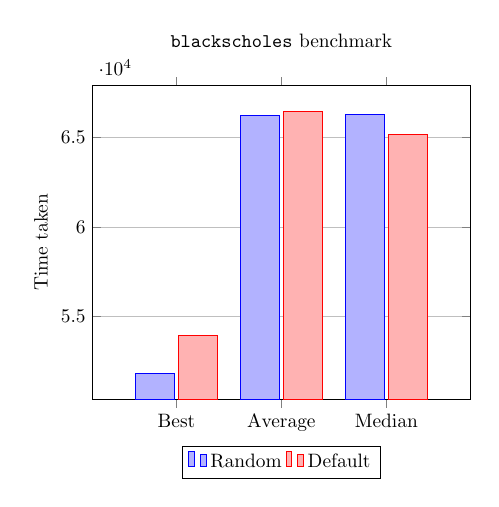
\begin{tikzpicture}[scale=0.7]
\begin{axis}[
    ybar,
    title={\texttt{blackscholes} benchmark},
   	title style={yshift=1em},
    bar width=2em,
    enlarge x limits=0.4,
    legend style={at={(0.5,-0.15)},
      anchor=north,legend columns=-1},
    ylabel={Time taken},
    symbolic x coords={Best,Average, Median},
    xtick=data,
    ymajorgrids=true, 
    ]
\addplot coordinates {(Best,51847) (Average,66251) (Median, 66284)};
\addplot coordinates {(Best,53932) (Average,66453) (Median, 65195)};
\legend{Random,Default}
\end{axis}
\end{tikzpicture}
\end{minipage}
%
\begin{minipage}{0.5\textwidth}
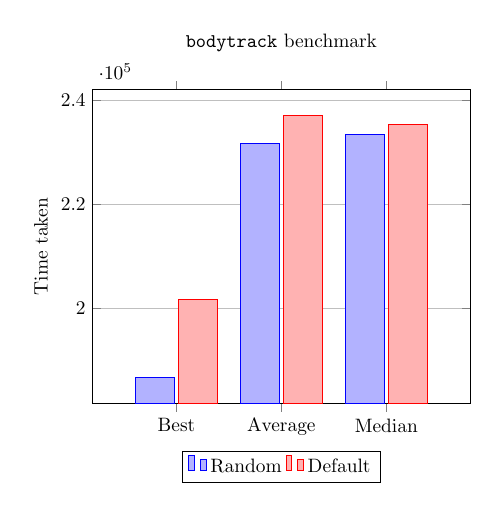
\begin{tikzpicture}[scale=0.7]
\begin{axis}[
    ybar,
    title={\texttt{bodytrack} benchmark},
   	title style={yshift=1em},
    bar width=2em,
    enlarge x limits=0.4,
    legend style={at={(0.5,-0.15)},
      anchor=north,legend columns=-1},
    ylabel={Time taken},
    symbolic x coords={Best,Average,Median},
    xtick=data,
    ymajorgrids=true,
    ]
\addplot coordinates {(Best,186594) (Average,231639) (Median, 233491)};
\addplot coordinates {(Best,201618) (Average,237037) (Median, 235465)};
\legend{Random,Default}
\end{axis}
\end{tikzpicture}
\end{minipage}
\caption{Best and average times taken by the random and default approach.}
\end{figure}
\noindent There are a few interesting points to note about the random and default approaches. First, the random approach is able to find a faster schedule than the default. This is interesting as one would expect the default approach to be able to come up with good and fast schedules. This shows that better schedules can be found through search that improve upon those made by the default scheduler. Following this, it can be seen that the average times for random and default are quite similar, though random more clearly outperforms for \texttt{bodytrack}. The median was also taken as an extra check to make sure the average was not skewed by anomalies, such as when the time taken is set to 0 for simulations which failed. This shows how the two approaches are similar in the kind of schedules being produced. An algorithm that can improve on a random approach should also improve against the default approach. 
\n
Another statistic of note is the variance, or standard deviation of the random and default approach. Here, the standard deviation is divided by the mean to get the variability relative to the mean and to be able to compare the two benchmarks.
\begin{figure}[H]
\centering
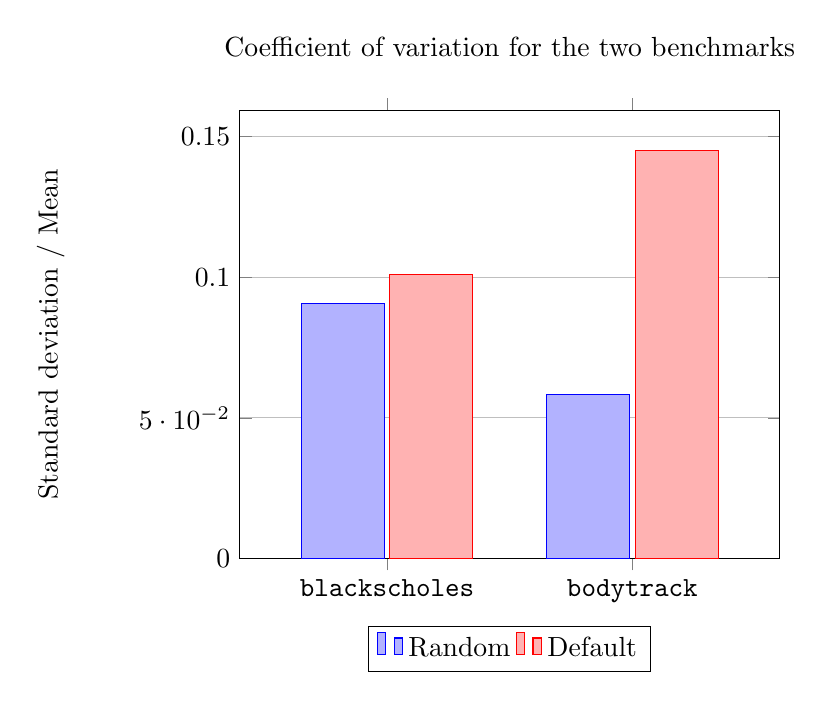
\begin{tikzpicture}
\begin{axis}[
    ybar,
    title={Coefficient of variation for the two benchmarks},
   	title style={yshift=1em},
    bar width=3em,
    enlarge x limits=0.6,
    legend style={at={(0.5,-0.15)},
      anchor=north,legend columns=-1},
    ymin=0,
    ylabel={Standard deviation / Mean},
    ylabel style={yshift=2em},
    symbolic x coords={\texttt{blackscholes},\texttt{bodytrack}},
    xtick=data,
    ymajorgrids=true,
    ]
\addplot coordinates {(\texttt{blackscholes},0.0906) (\texttt{bodytrack},0.05842)};
\addplot coordinates {(\texttt{blackscholes},0.101) (\texttt{bodytrack},0.14492)};
\legend{Random,Default}
\end{axis}
\end{tikzpicture}
\caption{Coefficient of variation by the random and default approach, showing sensitivity of the benchmarks to random changes in schedules.}
\label{fig:variance}
\end{figure}
\noindent Again, it can be seen that the variation in schedules for the default approach is not necessarily better than that of random schedules. This may be due to some mistake or assumption by the scheduler which led to slower schedules than expected. A certain approach by the scheduler may be very effective for other benchmarks, but less useful for these benchmarks. Additionally, in the \texttt{bodytrack} benchmark, the low variation for random yet high variation for the default suggests the benchmark may be less sensitive to random changes in the schedule. This means a smaller search space, as changes in the schedule have a smaller effect on the time taken.

\subsubsection{Genetic algorithm results}
Now the results for both genetic algorithm experiments described earlier will be analysed and compared. In theory, the systematic approach of the algorithm should result in better schedules, or at least a better method to guarantee getting good schedules. Something to keep in mind is that since the second experiment had a larger population, it is able to run more simulations per generation, which may skew results to its favour. 
\n
First, the difference between the two experiments are compared, to see if the changes made to the parameters of the first experiment had an effect. There are two anomalies in the data for the first experiment on \texttt{blackscholes}, where the time taken significantly decreased, but subsequent generations did not pick up or re-use this good schedule. This may be a fault of the machines, where the best schedule was lost on the next generation. Still, a general trend can be seen for both benchmarks. 
\begin{figure}[H]
\centering
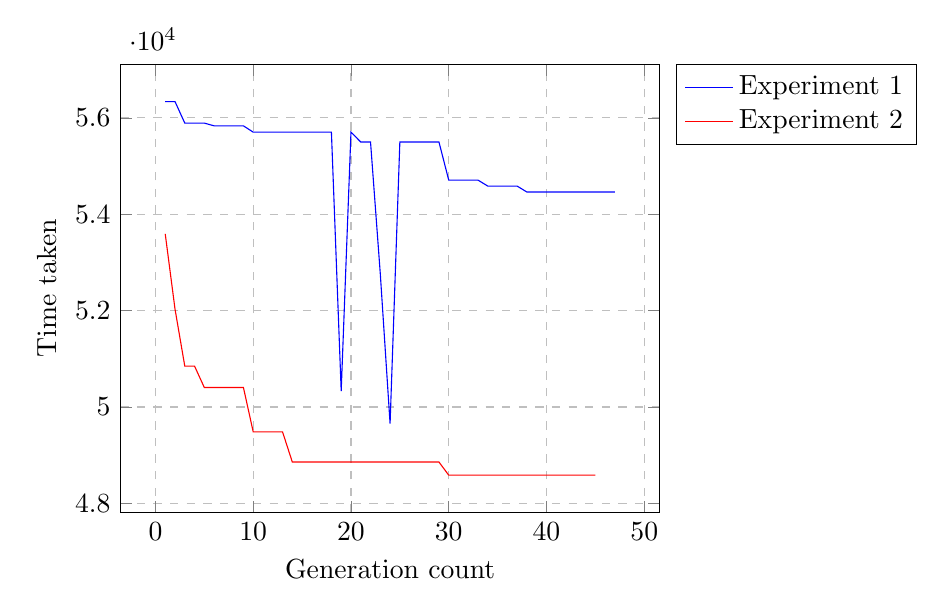
\begin{tikzpicture}
\begin{axis}[ 
    xlabel={Generation count},
    ylabel={Time taken},
    ymajorgrids=true,
    xmajorgrids=true,
    grid style=dashed,
    legend pos=outer north east,
] 
\addplot [color=blue, mark=circle,] coordinates {(1, 56339) (2, 56339) (3, 55892) (4, 55892) (5, 55892) (6, 55835) (7, 55835) (8, 55835) (9, 55835) (10, 55704) (11, 55704) (12, 55704) (13, 55704) (14, 55704) (15, 55704) (16, 55704) (17, 55704) (18, 55704) (19, 50331) (20, 55704) (21, 55500) (22, 55500) (23, 52763) (24, 49653) (25, 55500) (26, 55500) (27, 55500) (28, 55500) (29, 55500) (30, 54708) (31, 54708) (32, 54708) (33, 54708) (34, 54584) (35, 54584) (36, 54584) (37, 54584) (38, 54461) (39, 54461) (40, 54461) (41, 54461) (42, 54461) (43, 54461) (44, 54461) (45, 54461) (46, 54461) (47, 54461)};
\label{plot:blackscholes1}
\addlegendentry{Experiment 1}

\addplot [color=red, mark=circle,] coordinates {(1, 53593) (2, 52033) (3, 50848) (4, 50848) (5, 50403) (6, 50403) (7, 50403) (8, 50403) (9, 50403) (10, 49483) (11, 49483) (12, 49483) (13, 49483) (14, 48857) (15, 48857) (16, 48857) (17, 48857) (18, 48857) (19, 48857) (20, 48857) (21, 48857) (22, 48857) (23, 48857) (24, 48857) (25, 48857) (26, 48857) (27, 48857) (28, 48857) (29, 48857) (30, 48584) (31, 48584) (32, 48584) (33, 48584) (34, 48584) (35, 48584) (36, 48584) (37, 48584) (38, 48584) (39, 48584) (40, 48584) (41, 48584) (42, 48584) (43, 48584) (44, 48584) (45, 48584)};
\label{plot:blackscholes2}
\addlegendentry{Experiment 2}

\end{axis}
\end{tikzpicture}
\caption{Best times taken by the genetic algorithm experiments on the \texttt{blackscholes} benchmark}
\label{fig:scholes-ga-best}
\end{figure}

\begin{figure}[H]
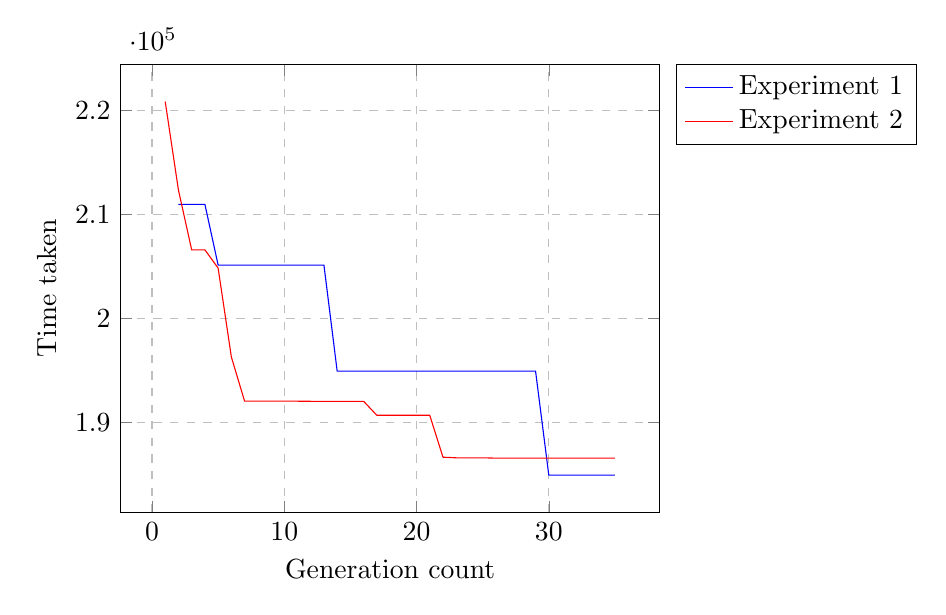
\begin{tikzpicture}
\begin{axis}[
    xlabel={Generation count},
    ylabel={Time taken},
    ymajorgrids=true,
    xmajorgrids=true,
    grid style=dashed,
    legend pos=outer north east,
] 
\addplot [color=blue, mark=circle,] coordinates {(2, 210986) (3, 210986) (4, 210986) (5, 205146) (6, 205146) (7, 205146) (8, 205146) (9, 205146) (10, 205146) (11, 205146) (12, 205146) (13, 205146) (14, 194954) (15, 194954) (16, 194954) (17, 194954) (18, 194954) (19, 194954) (20, 194954) (21, 194954) (22, 194954) (23, 194954) (24, 194954) (25, 194954) (26, 194954) (27, 194954) (28, 194954) (29, 194954) (30, 184958) (31, 184958) (32, 184958) (33, 184958) (34, 184958) (35, 184958)}; 
\label{plot:bodytrack1}
\addlegendentry{Experiment 1}

\addplot [color=red, mark=circle,] coordinates {(1, 220865) (2, 212348) (3, 206616) (4, 206616) (5, 204856) (6, 196318) (7, 192067) (8, 192067) (9, 192067) (10, 192067) (11, 192067) (12, 192056) (13, 192056) (14, 192056) (15, 192056) (16, 192056) (17, 190711) (18, 190711) (19, 190711) (20, 190711) (21, 190711) (22, 186685) (23, 186625) (24, 186625) (25, 186625) (26, 186594) (27, 186594) (28, 186594) (29, 186594) (30, 186594) (31, 186594) (32, 186594) (33, 186594) (34, 186594) (35, 186594)};
\label{plot:bodytrack2}
\addlegendentry{Experiment 2}


\end{axis}
\end{tikzpicture}
\caption{Best times taken by the genetic algorithm experiments on the \texttt{bodytrack} benchmark.}
\end{figure}
\noindent For \texttt{blackscholes}, the best schedules of the first experiment are clearly not as fast as those from the second experiment. The issue of diversity may have prevented the first experiment from getting out of a local maximum. By chance perhaps the first experiment could have found a better schedule, but it could not overcome being stuck. By contrast, the second set of parameters which increased the diversity of the populations seemed to be able to find faster schedules, but it is unclear whether this is due to the increased diversity, or if the mutation happened to be lucky. Both experiments had portions of generations where a better solution could not be found for a while, so it is not immediately obvious that increasing diversity is of great help to finding a better schedule. 
\n
The graphs for the \texttt{bodytrack} experiment support the claim that the parameters and diversity have little effect, as both experiments were able to continue finding better schedules. However, it could be the case that the first experiment got lucky. To be able to show the effect of the genetic algorithm parameters on the ability and consistency to find good schedules, more trials of the experiments would have had to be run to show these cases are not simply one-offs. If the diversity does have an affect, the expected results of more trials on experiment one would be finding some trials with good schedules and others where the local maximum is stuck somewhere far from a good time. The second experiment should then consistently end up with a good schedule every trial. Running more trials can also give further insight into how the properties of the benchmarks could have an affect, as perhaps both experiments perform similarly on one benchmark but differently on another. For example since \texttt{bodytrack} seems less sensitive to random changes, increased diversity from experiment 2 may have less effect and therefore perform similarly to experiment 1. 
\n
The two experiments can also be compared by how their average time taken changes for each generation. This will show how the entire population of the genetic algorithm tends towards good schedules with each subsequent population.
\begin{figure}[H]
\begin{minipage}{0.5\textwidth}
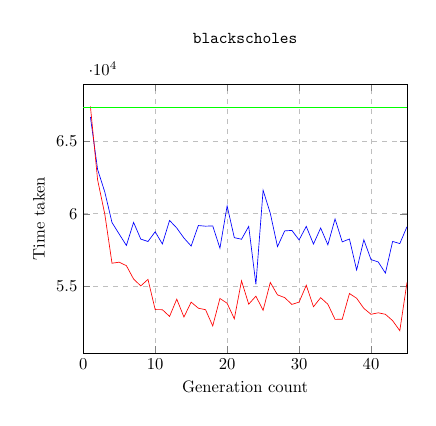
\begin{tikzpicture}[scale=0.6]
\begin{axis}[
	title={\texttt{blackscholes}},
	title style={yshift=1.5em},
    xlabel={Generation count},
    ylabel={Time taken},
    xmin=0,
    xmax=45,
    ymajorgrids=true,
    xmajorgrids=true,
    grid style=dashed,
    legend style={font=\fontsize{14}{6}\selectfont},
    legend pos=outer north east,
] 
\addplot [color=blue, mark=circle,] coordinates {(1, 66634.44) (2, 63035.5) (3, 61486) (4, 59395) (5, 58602.12) (6, 57823.57) (7, 59404.64) (8, 58258) (9, 58093.80) (10, 58761.12) (11, 57925) (12, 59540) (13, 59018.52) (14, 58331) (15, 57783) (16, 59189.88) (17, 59144.2) (18, 59165.48) (19, 57634) (20, 60534.88) (21, 58357.64) (22, 58248.84) (23, 59130) (24, 55154) (25, 61612.44) (26, 60029) (27, 57741) (28, 58823) (29, 58856) (30, 58200) (31, 59129.2) (32, 57918.16) (33, 59019) (34, 57868) (35, 59641) (36, 58069.2) (37, 58266) (38, 56136) (39, 58209) (40, 56852.36) (41, 56692) (42, 55925) (43, 58099.28) (44, 57950) (45, 59109.36)}; 
\label{plot:bodytrack1-stdev}

\addplot [color=red, mark=circle,] coordinates {(1, 67355.8) (2, 62320.85) (3, 59967) (4, 56603.05) (5, 56674.95) (6, 56435) (7, 55519.25) (8, 55046) (9, 55496) (10, 53423.525) (11, 53415) (12, 52954) (13, 54138.475) (14, 52910) (15, 53934) (16, 53518) (17, 53414) (18, 52301) (19, 54186) (20, 53856) (21, 52791) (22, 55395) (23, 53793.55) (24, 54342.925) (25, 53375) (26, 55284.375) (27, 54432.2) (28, 54245) (29, 53776.675) (30, 53935) (31, 55089.15) (32, 53616.825) (33, 54239.925) (34, 53790.275) (35, 52750) (36, 52761.95) (37, 54524.45) (38, 54200.35) (39, 53506) (40, 53098.5) (41, 53202) (42, 53099) (43, 52662.025) (44, 51975.825) (45, 55287.95)};
\label{plot:bodytrack2-stdev}

\addplot [color=green, mark=circle,] coordinates {(0, 67325) (45, 67325)};
\label{plot:bodytrack-random}

\end{axis}
\end{tikzpicture}
\end{minipage}
%
\begin{minipage}{0.5\textwidth}
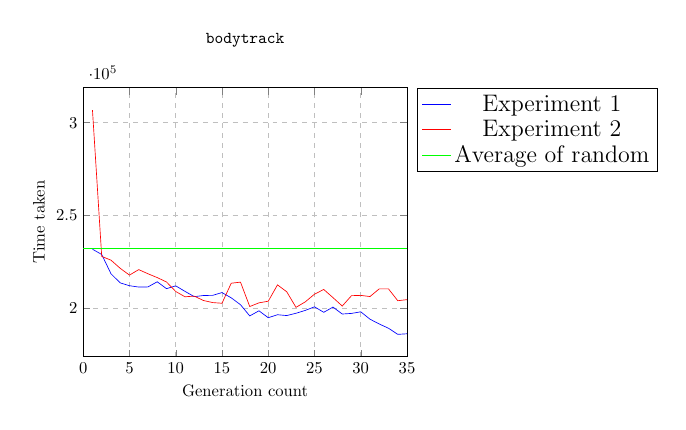
\begin{tikzpicture}[scale=0.6]
\begin{axis}[
	title={\texttt{bodytrack}},
	title style={yshift=1.5em},
    xlabel={Generation count},
    ylabel={Time taken},
    xmin=0,
    xmax=35,
    ymajorgrids=true,
    xmajorgrids=true,
    grid style=dashed,
    legend style={font=\fontsize{14}{6}\selectfont},
    legend pos=outer north east,
] 
\addplot [color=blue, mark=circle,] coordinates {(1, 231860) (2, 229007.88) (3, 218628) (4, 213711) (5, 212184) (6, 211468.75) (7, 211545.6) (8, 214313) (9, 210605.76) (10, 212104.24) (11, 209150.12) (12, 206299) (13, 206915) (14, 207009) (15, 208497) (16, 205663) (17, 201958) (18, 195927.32) (19, 198685.08) (20, 194954) (21, 196567) (22, 196107.44) (23, 197356.84) (24, 198886.64) (25, 200816) (26, 197869) (27, 200676.16) (28, 196945) (29, 197271.2) (30, 198136) (31, 194157.32) (32, 191576.88) (33, 189287.64) (34, 185991) (35, 186304)}; 
\label{plot:bodytrack1-stdev}
\addlegendentry{Experiment 1}

\addplot [color=red, mark=circle,] coordinates {(1, 306714) (2, 227957) (3, 225956.275) (4, 221548.6) (5, 217905) (6, 220861.4) (7, 218618.975) (8, 216569.2) (9, 214210) (10, 209076) (11, 206232.55) (12, 206578.975) (13, 204224) (14, 203101.05) (15, 202741.275) (16, 213535) (17, 214123.85) (18, 200974) (19, 202967.225) (20, 203836.075) (21, 212641) (22, 208925.275) (23, 200539.25) (24, 203474.8) (25, 207635.1) (26, 210162) (27, 205774) (28, 201236) (29, 206833.95) (30, 206980.8) (31, 206351) (32, 210508.9) (33, 210484.35) (34, 204121) (35, 204678.625)};
\label{plot:bodytrack2-stdev}
\addlegendentry{Experiment 2}

\addplot [color=green, mark=circle,] coordinates {(0, 232141) (35, 232141)};
\label{plot:bodytrack-random}
\addlegendentry{Average of random}

\end{axis}
\end{tikzpicture}
\end{minipage}
\caption{Mean time taken in each generation compared to the average time taken from all random runs.}
\label{plot:average-ga}
\end{figure}
\noindent Figure \ref{plot:average-ga} shows the two experiments getting better schedules on average for each generation. The line of average time taken by random schedules serves as a comparison. It is a straight line to represent the average random schedule. This suggests that the logic of the genetic algorithms can apply to this search problem. For each subsequent generation, the performance of the previous generations has affected the schedules created, resulting in getting better average schedules each generation compared to a random approach. This shows the genetic algorithms will guarantee getting better schedules after each generation as the entire population tends towards better schedules over time. The search space therefore is being traversed in a methodical way as described earlier in section \ref{sec:ga}. \texttt{blackscholes} has a larger search space compared to \texttt{bodytrack} which may explain the trend being not very clear. The mixture of selection, crossover and mutation seem to work in being able to keep strong schedules while mutating new children to try and improve the schedules. For further work, the mutation rate of each gene can be looked into. It would be expected that mutating more of the later genes affects searching through the current local maximum while mutating early genes would find new schedules. The overall effect should also be weaker for \texttt{bodytrack} as it is less responsive to changes in the schedule.
\n
Although this shows the genetic algorithm working for searching through the schedule space and will eventually lead to good schedules, it is not clear if this is a fast method of searching compared to the purely random approach. What is important is how fast the best schedule is for each generation, not the average time taken for the entire population. Compared to a purely random approach, the genetic algorithm may take more simulations just to guarantee a good schedule that the random approach can find by chance.
\begin{figure}[H]
\begin{minipage}{0.5\textwidth}
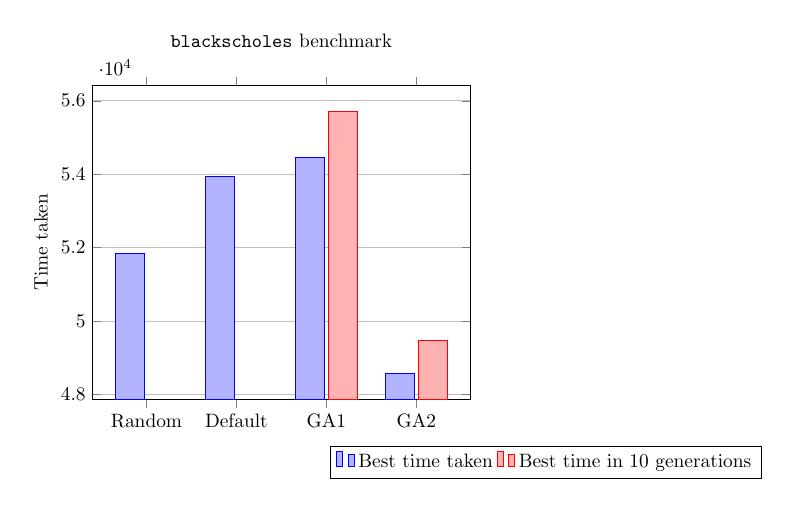
\begin{tikzpicture}[scale=0.7]
\begin{axis}[
    ybar,
    title={\texttt{blackscholes} benchmark},
   	title style={yshift=1em},
    bar width=1.5em,
    enlarge x limits=0.2,
    legend style={at={(1.2,-0.15)},
      anchor=north,legend columns=-1},
    ylabel={Time taken},
    symbolic x coords={Random,Default,GA1, GA2},
    xtick=data,
    ymajorgrids=true, 
    ]
\addplot coordinates {(Random,51847) (Default,53932) (GA1, 54461) (GA2, 48584)};
\addlegendentry{Best time taken};
\addplot coordinates {(GA1, 55704) (GA2, 49483)};
\addlegendentry{Best time in 10 generations};
\end{axis}
\end{tikzpicture}
\end{minipage}
%
\begin{minipage}{0.5\textwidth}
\begin{tikzpicture}[scale=0.7]
\begin{axis}[
    ybar,
    title={\texttt{bodytrack} benchmark},
   	title style={yshift=1em},
    bar width=1.5em,
    enlarge x limits=0.2,
    legend style={at={(11,-0.15)},
      anchor=north,legend columns=-1},
    ylabel={Time taken},
    symbolic x coords={Random,Default,GA1, GA2},
    xtick=data,
    ymajorgrids=true, 
    ]
\addplot coordinates {(Random,186594) (Default,201618) (GA1, 184958) (GA2, 186594)};
\addlegendentry{};
\addplot coordinates {(GA1, 205146) (GA2, 192067)};
\end{axis}
\end{tikzpicture}
\end{minipage}
\caption{Best times taken by all approaches.}
\label{plot:best-all}
\end{figure}
\noindent The best time taken for every approach is compared in figure \ref{plot:best-all}. The best time taken for the first genetic algorithm experiment does not take into account the outliers that could be seen in figure \ref{fig:scholes-ga-best} to be able to show the general trend that the experiment was exhibiting. 
\n
When comparing all the approaches, it is not clear if the genetic algorithms perform better at finding good schedules compared to the random approach. The red bars represent the best schedule found in only 10 generations, which is important for a proper comparison, as the genetic algorithms were allowed to run for more simulations compared to the default and random schedules. We see the genetic algorithms sometimes find better schedules, but not all the time and especially not with a comparable number of simulations. Given more time to run more experiments, the parameters for the genetic algorithm could be improved and analysed to find an optimal version where it converges to good schedules faster while maintaining diversity. The size of the search space also seems to affect the effectiveness of the genetic algorithm. For example in \texttt{blackscholes}, the second experiment is able to find a very good schedule compared to random and experiment 1 whereas random outperforms both genetic algorithm experiments for \texttt{bodytrack}. It was suggested earlier that \texttt{bodytrack} has a smaller search space due to how the variation of random schedules is small. This perhaps shows the genetic algorithm performing better for a larger search space, where it can methodically find peaks. In a smaller search space, the random is likely to be able to find a good schedule faster and before the genetic algorithms can converge to some maximum. This can be shown more clearly if a larger variety of benchmarks and more trials for every benchmark were run. 
\n
The difference between the genetic algorithm and random approach represents a trade-off in searching for fast schedules as well as how big of a space needs to be searched. If it is required under some constraint to find good schedule, or the optimisation space is quite large, it may be better to use an optimised genetic algorithm to guarantee a good schedule. However, if there are less constraints and a smaller search space, running random schedules can have a good chance to find something better in less simulations, but it is not guaranteed.

\subsection{Conclusion}
In conclusion, the genetic algorithm implemented was able to find better schedules as the number of generations increase and is able to improve upon the default scheduler. It works on crossing over good parent schedules with mutation to both avoid local maximum and use the parent's genes to try and get something better. However, when compared to randomly searching for schedules, the genetic algorithm was not very efficient with the number of simulations needed. 
\n
A random approach is able to find a comparable schedule in the same number of simulations as the genetic algorithm. This also depends on the size of the search space as a random search on a large space will be less effective. The advantage of the genetic algorithm is that the whole population will tend to a better schedule, so it is guaranteed to find something better than the default and it is able to more systematically search through larger spaces. A good schedule is not guaranteed for the random approach, but the smaller the search space, the more likely a good random schedule can be found.

\printbibliography

\end{document}



